 \documentclass[a4paper,10pt]{article}
\input{/Users/WannaGetHigh/workspace/latex/macros.tex}

\title{IHM - TP: jTunes}
\author{Fran�ois \bsc{Lepan} - Benjamin \bsc{Van Ryseghem}}

\begin{document}
\maketitle

\section*{Introduction}

Ce rapport d�crit la conception et l'utilisation d'un lecteur mp3. Nous verrons tout d'abord comment utiliser ce lecteur et ensuite nous verrons la conception de celui-ci.

\section{Le lecteur jTunes}

\begin{figure}[ht]
\begin{center}
	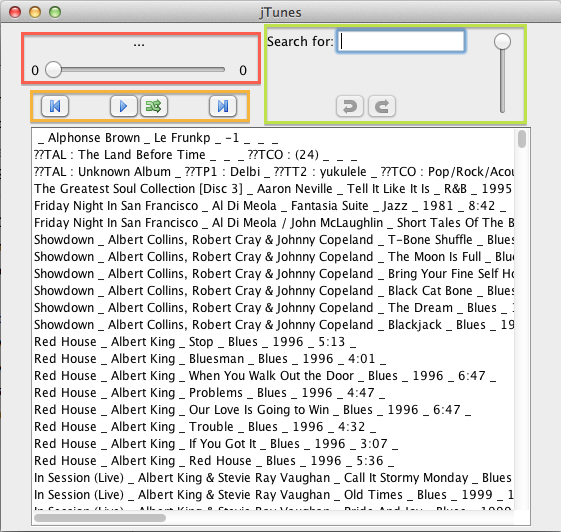
\includegraphics[width=10cm]{figures/jTunes.png}
\end{center}
	\caption{Le lecteur mp3 jTunes}
	\label{lecteur_mp3}
\end{figure}

On retrouve dans ce lecteur (\emph{c.f.} ~Fig.~\ref{lecteur_mp3}) plusieurs zones. La premi�re (en rouge) est compos�e d'un curseur permettant de savoir o� en est la music lors de la lecture et de changer la position de la lecture. � cot� de ce curseur on retrouve des labels indiquant la dur�e �coul�e, le temps restant ainsi que le nom de la chanson jou� au dessus du curseur.

En dessous (orange) on retrouve les boutons "lecture/pause", "next", "pr�c�dent" et "al�atoire" qui permettent de changer les musiques jou�es.

� droite (vert) on retrouve la bar de recherche, en dessous deux boutons "annuler" et "refaire" permettant d'annuler ou refaire la derni�re action et � droite de ceux-ci se trouve le curseur permettant de g�rer le son.

En dessous de ces �l�ments on retrouve la liste de music, qui affiche les informations des titres pr�sent dans la base de donn�e.

\section{Impl�mentation}

Ce lecteur mp3 � �t� con�u sur la base d'un MVC. Nous avons g�n�r� l'UML au sein de la JavaDoc car nous pensons que ce sera plus facile pour comprendre les classes impl�ment�es. 

Nous avons rajouter un "Undo/Redo" ainsi qu'un drag and drop pour la liste de music. Nous pensons que cela permettra � l'utilisateur une meilleur exp�rience avec le lecteur. En effet il peut changer l'ordre de lecture et si cela ne lui plait pas il pourra annuler le changement effectuer.

Nous avons aussi un double dispatch sur les actions du "undo/redo".

\section*{Conclusion}


Ce Lecteur permet de lire des music visualiser une liste de lecture et �diter cette liste de lecture et permettre � l'utilisateur une bonne exp�rience.


\end{document}